\documentclass[]{book}
\usepackage{lmodern}
\usepackage{amssymb,amsmath}
\usepackage{ifxetex,ifluatex}
\usepackage{fixltx2e} % provides \textsubscript
\ifnum 0\ifxetex 1\fi\ifluatex 1\fi=0 % if pdftex
  \usepackage[T1]{fontenc}
  \usepackage[utf8]{inputenc}
\else % if luatex or xelatex
  \ifxetex
    \usepackage{mathspec}
  \else
    \usepackage{fontspec}
  \fi
  \defaultfontfeatures{Ligatures=TeX,Scale=MatchLowercase}
\fi
% use upquote if available, for straight quotes in verbatim environments
\IfFileExists{upquote.sty}{\usepackage{upquote}}{}
% use microtype if available
\IfFileExists{microtype.sty}{%
\usepackage{microtype}
\UseMicrotypeSet[protrusion]{basicmath} % disable protrusion for tt fonts
}{}
\usepackage[margin=1in]{geometry}
\usepackage{hyperref}
\hypersetup{unicode=true,
            pdftitle={Biology 3103 - Ecology Laboratory},
            pdfauthor={S Cook},
            pdfborder={0 0 0},
            breaklinks=true}
\urlstyle{same}  % don't use monospace font for urls
\usepackage{natbib}
\bibliographystyle{apalike}
\usepackage{longtable,booktabs}
\usepackage{graphicx,grffile}
\makeatletter
\def\maxwidth{\ifdim\Gin@nat@width>\linewidth\linewidth\else\Gin@nat@width\fi}
\def\maxheight{\ifdim\Gin@nat@height>\textheight\textheight\else\Gin@nat@height\fi}
\makeatother
% Scale images if necessary, so that they will not overflow the page
% margins by default, and it is still possible to overwrite the defaults
% using explicit options in \includegraphics[width, height, ...]{}
\setkeys{Gin}{width=\maxwidth,height=\maxheight,keepaspectratio}
\IfFileExists{parskip.sty}{%
\usepackage{parskip}
}{% else
\setlength{\parindent}{0pt}
\setlength{\parskip}{6pt plus 2pt minus 1pt}
}
\setlength{\emergencystretch}{3em}  % prevent overfull lines
\providecommand{\tightlist}{%
  \setlength{\itemsep}{0pt}\setlength{\parskip}{0pt}}
\setcounter{secnumdepth}{5}
% Redefines (sub)paragraphs to behave more like sections
\ifx\paragraph\undefined\else
\let\oldparagraph\paragraph
\renewcommand{\paragraph}[1]{\oldparagraph{#1}\mbox{}}
\fi
\ifx\subparagraph\undefined\else
\let\oldsubparagraph\subparagraph
\renewcommand{\subparagraph}[1]{\oldsubparagraph{#1}\mbox{}}
\fi

%%% Use protect on footnotes to avoid problems with footnotes in titles
\let\rmarkdownfootnote\footnote%
\def\footnote{\protect\rmarkdownfootnote}

%%% Change title format to be more compact
\usepackage{titling}

% Create subtitle command for use in maketitle
\newcommand{\subtitle}[1]{
  \posttitle{
    \begin{center}\large#1\end{center}
    }
}

\setlength{\droptitle}{-2em}
  \title{Biology 3103 - Ecology Laboratory}
  \pretitle{\vspace{\droptitle}\centering\huge}
  \posttitle{\par}
  \author{S Cook}
  \preauthor{\centering\large\emph}
  \postauthor{\par}
  \predate{\centering\large\emph}
  \postdate{\par}
  \date{Summer 2018}

\usepackage{booktabs}

\usepackage{amsthm}
\newtheorem{theorem}{Theorem}[chapter]
\newtheorem{lemma}{Lemma}[chapter]
\newtheorem{corollary}{Corollary}[chapter]
\newtheorem{proposition}{Proposition}[chapter]
\newtheorem{conjecture}{Conjecture}[chapter]
\theoremstyle{definition}
\newtheorem{definition}{Definition}[chapter]
\theoremstyle{definition}
\newtheorem{example}{Example}[chapter]
\theoremstyle{definition}
\newtheorem{exercise}{Exercise}[chapter]
\theoremstyle{remark}
\newtheorem*{remark}{Remark}
\newtheorem*{solution}{Solution}
\begin{document}
\maketitle

{
\setcounter{tocdepth}{1}
\tableofcontents
}
\chapter{Population Ecology}\label{week1}

\section{Exploration of life history strategies with population
demography}\label{exploration-of-life-history-strategies-with-population-demography}

Organisms have evolved different life history strategies which differ in
their methods of reproduction, care of offspring, timing of growth,
means of resource acquisition, and prey avoidance. While these factors
and how they interact can be highly complex, \textbf{survivorship}
offers a simple means to quantify how a particular population ensures
their reproductive success. For example, humans devote an enormous
amount of energy and resources to offspring care, which results in low
mortality rates among their young. On the other hand, most insects
produce a massive number of offspring that have extremely high rates of
mortality.

Plotting the number of survivors against age yields what is called a
`survivorship-curve' (Fig. \ref{fig:survivor-fig}), which is a visual
way to assess how various organisms differ in their \textbf{life-history
strategies} (number of offspring, number of reproductive cycles, degree
of parental care, etc.). Scientists can use these plots to examine
differences in organisms, or assess changes within subsets of a
population.

\begin{figure}
\centering
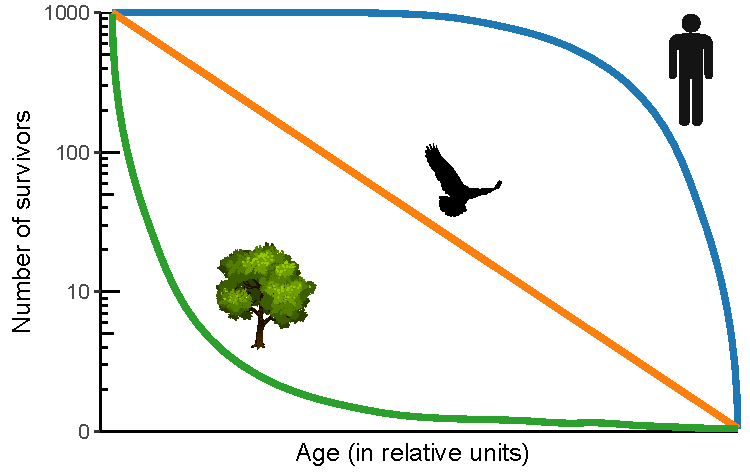
\includegraphics{../Population_ecology_material/base_plot.pdf}
\caption{\label{fig:survivor-fig}Idealized examples of Types I, II, and III
survivorship curves overlaid with example organisms. Type I survivorship
is characterized by high probability of survival early in life, followed
by a rapid decline as individuals reach older age. Type II survivorship
displays roughly constant mortality throughout the lifespan of the
organism, and Type III exhibits high mortality among young offspring.}
\end{figure}

\section{Objectives}\label{objectives}

You will use the cemetery data, as well as data generated by the U.S.
Fish \& Wildlife Service \citep{milsap_bald_2016}, to address hypotheses
about different populations. We can use birth and death years on
gravestones, as well as names (to infer gender), to collect simple but
useful information to collect demographic data for the local human
population. The survivorship curve you will generate from this data will
inform some ideas about the life history strategy of humans.

Additionally, survey data collected by state and federal agencies
provide valuable information about natural population. We can use
ancillary data about individuals within a population to examine how
different forces influence demographics within a population. Golden
Eagles are federally protected in the United States, and Fish \&
Wildlife collects detailed information from tagged individuals (Fig.
\ref{fig:eagle-fig}).

\begin{figure}
\centering
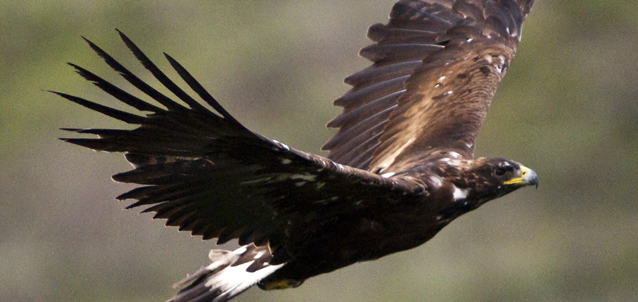
\includegraphics{../Population_ecology_material/golden_eagle.jpg}
\caption{\label{fig:eagle-fig}Migratory Golden eagle in Denali National Park
\& Preserve. Mating pairs return each year to northern nesting territory
in the spring, and most new fledglings leave the nest by mid-August.
During winter their range extends from southern Canada to south of the
Rocky Mountains \citep{brown_patterns_2017}.}
\end{figure}

We will use this data to test hypotheses addressing the following
questions:

\begin{enumerate}
\def\labelenumi{\arabic{enumi}.}
\tightlist
\item
  Do humans and eagles display different life history strategies?
\item
  Does gender affect survivorship in human populations?

  \begin{itemize}
  \tightlist
  \item
    And if so, how?
  \end{itemize}
\item
  Does human impact affect survivorship in eagle populations?

  \begin{itemize}
  \tightlist
  \item
    And if so, how?
  \end{itemize}
\end{enumerate}

Please form testable null hypotheses to address question number 1 and
\textbf{either} question 2 or 3 (pick one). If you want, you may also
substitute question 2 or 3 to address a hypothesis using the extra data
we generated from the gravestones (height of gravestones as a proxy of
material wealth).

To evaluate your hypotheses, you will\ldots{}

\begin{enumerate}
\def\labelenumi{\arabic{enumi}.}
\tightlist
\item
  Statistically address differences in survivorship between groups using
  a \textbf{t-test}, and display that information using a
  \textbf{bar-graph}
\item
  Unpack question 1 by \textbf{computing} and \textbf{displaying
  survivorship} (no statistical test needed for this part).
\end{enumerate}

\section{Data Analysis}\label{data-analysis}

\begin{enumerate}
\def\labelenumi{\arabic{enumi}.}
\tightlist
\item
  Calculate the age at death of every individuals in both data sets
\item
  If necessary, use Excel to sort (Google it) the data based on your
  column of interest (i.e.~gender).

  \begin{itemize}
  \tightlist
  \item
    Sorting the data easily splits the population into groups that you
    can then run the calculations (below) on. If you are doing the
    entire population, you will not need to split the population, but
    for within-population questions this step will come in handy. Keep
    in mind that every time you split the data based on a categorical
    variable, you will normalize to a hypothetical population of 1000
    for the survivorship plots below.
  \end{itemize}
\item
  Calculate mean age at death, as well as a measure of variation around
  that mean for use in the \textbf{bar-graphs}.

  \begin{itemize}
  \tightlist
  \item
    The \textbf{bar-graph} is just a visual representation of the data.
    You will perform a \textbf{t-test} on this data and report the
    results to determine if the population means are actually different.
  \end{itemize}
\item
  Create a survivorship table

  \begin{itemize}
  \tightlist
  \item
    Create ``bins'' of individuals

    \begin{itemize}
    \tightlist
    \item
      0 to 1, 1 to 2, 2 to 3, etc\ldots{} for Golden Eagles
    \item
      0-9, 10-19, 20-29, etc\ldots{} for humans
    \end{itemize}
  \item
    Calculate the number of individuals surviving to that age class (the
    `countif' function in Excel will come in handy here). Keep in mind
    that for the first group you will want to count \textbf{all} of the
    observations in the data set, so your condition will be
    `\textgreater{}=0'.
  \item
    Normalize survivors to a hypothetical population of 1000

    \begin{itemize}
    \tightlist
    \item
      This will make comparisons possible between unequal sample -- so
      if you have 1250 observations in the data set, your normalized
      number for the first age class will be 1250/1250 = 1.0, which is a
      proportion you can multiply by 1000. For the second age class (if
      you have some mortality), it might be 975/1250 = 0.78, which you
      can then multiply by 1000 which equals 780.
    \end{itemize}
  \end{itemize}
\item
  Plot the number of survivors (y-axis values) against age class (x-axis
  values) to construct the survivorship curves. You may plot the data
  from the survivorship table either as normalized survivors, or on a
  logarithmic x-axis (typically how this data is displayed, as in Fig.
  \ref{fig:survivor-fig}).
\end{enumerate}

The procedure above will ultimately yield survivorship (number of
surviving individuals at a particular age class), which you may plot to
visually explore differences between groups of interest to you.

\section{Lab Report Specifics}\label{lab-report-specifics}

Below are some specific guidelines for this lab report, but you should
also utilize the general grading rubric in the Syllabus!

\begin{itemize}
\item
  \textbf{Participation} (1 pts)
\item
  \textbf{Introduction} (3 pts)

  \begin{itemize}
  \tightlist
  \item
    General information about population ecology / life history
    strategies
  \item
    How are survivorship curves used in population ecology?
  \item
    Build up rationale to lead into your objectives/hypotheses
    statements.
  \end{itemize}
\item
  \textbf{Methods} (3 pts)

  \begin{itemize}
  \tightlist
  \item
    Explanation of data collection and analysis
  \end{itemize}
\item
  \textbf{Results} (6 pts)

  \begin{itemize}
  \tightlist
  \item
    Summary statistics in the text
  \item
    Bar-plots and associated t-tests for each question
  \item
    Survivorship curves for each question
  \end{itemize}
\item
  \textbf{Discussion} (3 pts)

  \begin{itemize}
  \tightlist
  \item
    Explain your results in light of your hypotheses
  \item
    What are some plausible explanations for differences (or lack
    thereof) between groups?
  \item
    Place your results in an evolutionary context.
  \end{itemize}
\end{itemize}

\bibliography{book.bib,packages.bib}


\end{document}
